\card{
  What do we do here?\\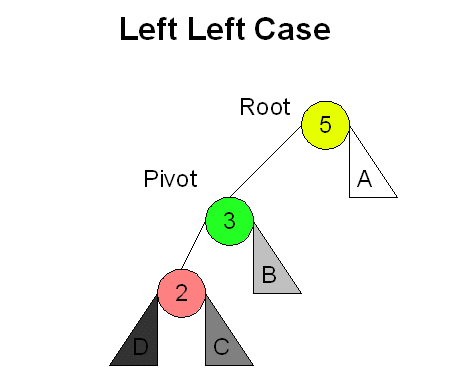
\includegraphics[height=0.8\cardheight]{images/left-left}
}{
  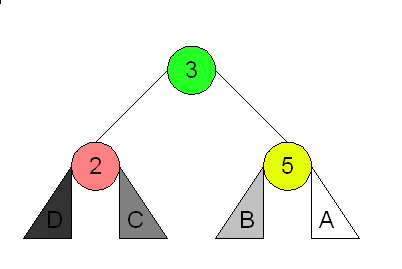
\includegraphics[height=0.8\cardheight]{images/left-left-out}
}

\card{
  What do we do here?\\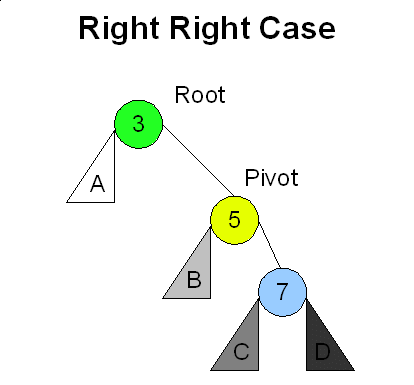
\includegraphics[height=0.8\cardheight]{images/right-right}
}{
  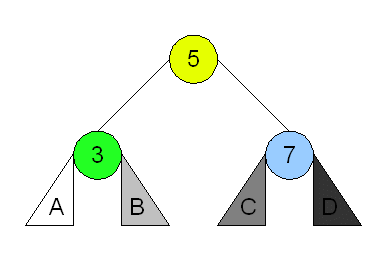
\includegraphics[height=0.8\cardheight]{images/right-right-out}
}

\card{
  What do we do here?\\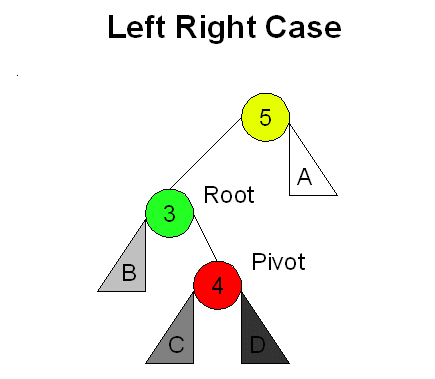
\includegraphics[height=0.8\cardheight]{images/left-right}
}{
  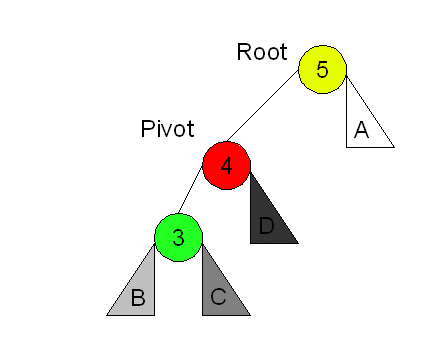
\includegraphics[height=0.8\cardheight]{images/left-right-mid}\\
  Then a left-left!
}

\card{
  What do we do here?\\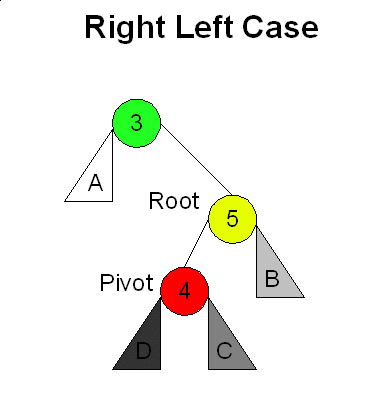
\includegraphics[height=0.8\cardheight]{images/right-left}
}{
  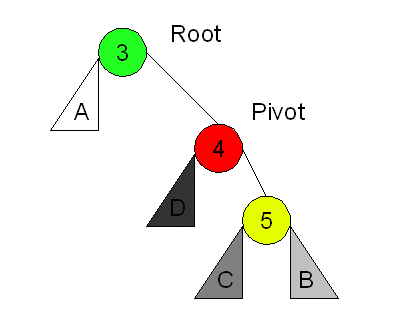
\includegraphics[height=0.8\cardheight]{images/right-left-mid}\\
  Then a right-right!
}

\card{
  What does a Depth First Search use?
}{
  A stack!
}

\card{
  What does a Breadth First Search use?
}{
  A queue!
}

\card{
  What is the running time of Dijkstra's algorithm?
}{
  $O(E + V\log(v))$
}

\card{
  What's the running time of a depth first search when the graph is an adjacency
  matrix?
}{
  $O(V^2)$ since finding neighbours takes $O(V)$ time.
}

\card{
  What's the running time of a depth first search when the graph is an adjacency
  list?
}{
  $O(V + E)$
}

\card{
  How do we insert an element into a heap?
}{
  First, you insert it at the next space in the heap (last element of current
  row, or a new row), then you keep swapping it with its parent if the parent
  is larger than it.
}

\card{
  How do we remove the smallest element from a (min) heap?
}{
  We move the last element from the heap to the first element (we can override
  the first element since we've removed it). Now we `down heap' by swapping
  the moved node with its smallest child until it is smaller than both its
  children or it has no children.
}